\documentclass{article}
\usepackage{amsmath}
\usepackage{amssymb}
\usepackage{graphicx}
\usepackage{hyperref}
\usepackage[version=4]{mhchem}


\begin{document}
\section*{Problem}
Find the length of the chord which is the perpendicular bisector of radius of length 24 in a circle.\\
(A) \(6 \sqrt{3}\)\\
(B) 54\\
(C) \(12 \sqrt{3}\)\\
(D) \(24 \sqrt{3}\)\\
(E) \(24 \sqrt{2}\)

\section*{Solution}
(D).\\
\(O\) is the center of the circle and \(O R\) is the radius. \(A B\) is the chord that is perpendicular bisectors of \(O R\), and \(A B\) and \(A R\) bisect each other at \(M\).\\
Applying the Pythagorean theorem to right triangle \(O M A\), we get \((A M)^{2}=(O A)^{2}-(O M)^{2}=24^{2}-12^{2}=432, A M=12 \sqrt{3}\).\\
\centering
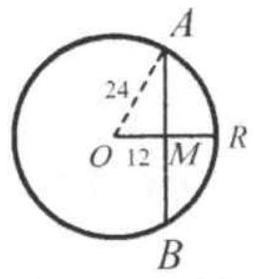
\includegraphics[width=\textwidth]{images/159(1).jpg}

Thus the length of the chord is \(2 \times 12 \sqrt{3}=24 \sqrt{3}\).\\

\end{document}
